\documentclass[11pt,a4paper]{article}

\usepackage[utf8]{inputenc}
\usepackage[T1]{fontenc}
\usepackage{subcaption}
\usepackage{array}
\usepackage{geometry}
\usepackage{amsmath}
\usepackage{booktabs}
\usepackage{graphicx}
\usepackage[normalem]{ulem}
\useunder{\uline}{\ul}{}
\usepackage{parskip}
\usepackage{enumitem}
\usepackage{microtype}
\usepackage{lmodern}
\usepackage{fancyhdr}
\usepackage{titlesec}
\usepackage[hyphens]{url}
\usepackage{tcolorbox}
\usepackage{listings}
\usepackage{xcolor}
\usepackage{longtable}
\usepackage{colortbl}
\usepackage{tikz}
\usetikzlibrary{arrows.meta} % Esta librería es la que contiene 'Stealth'
\usepackage{caption}
\usepackage{float}
\usepackage{hyperref}
\usepackage{tikz}
\setlength{\emergencystretch}{3em}
\usepackage[spanish]{babel}

% Definición de colores
\definecolor{codegreen}{rgb}{0,0.6,0}
\definecolor{codegray}{rgb}{0.5,0.5,0.5}
\definecolor{codepurple}{rgb}{0.58,0,0.82}
\definecolor{backcolour}{rgb}{0.95,0.95,0.92}

% Configuración del estilo para Python
\lstdefinestyle{estiloPython}{
    backgroundcolor=\color{backcolour},   
    commentstyle=\color{codegreen},
    keywordstyle=\color{magenta},
    numberstyle=\tiny\color{codegray},
    stringstyle=\color{codepurple},
    basicstyle=\ttfamily\footnotesize,
    breakatwhitespace=false,         
    breaklines=true,                 
    captionpos=b,                    
    keepspaces=true,                 
    numbers=left,                    
    numbersep=5pt,                  
    showspaces=false,                
    showstringspaces=false,
    showtabs=false,                  
    tabsize=4,
    language=Python,
    % Soporte para tildes y eñes en los comentarios
    extendedchars=true,
    literate={á}{{\'a}}1 {é}{{\'e}}1 {í}{{\'i}}1 {ó}{{\'o}}1 {ú}{{\'u}}1 {ñ}{{\~n}}1 {Á}{{\'A}}1 {É}{{\'E}}1 {Í}{{\'I}}1 {Ó}{{\'O}}1 {Ú}{{\'U}}1 {Ñ}{{\~N}}1
}

\lstset{style=estiloPython}

\geometry{margin=2.5cm}

\hypersetup{
    colorlinks=true,
    linkcolor=black,
    urlcolor=blue,
    citecolor=black
}

\pagestyle{fancy}
\fancyhf{}
\rhead{MINE4201 -- Sistemas de Recomendación}
\lhead{Taller 2}
\rfoot{\thepage}

\titleformat{\section}{\large\bfseries}{}{0em}{}[\titlerule]
\titleformat{\subsection}{\normalsize\bfseries}{}{0em}{}

\setlength{\headheight}{13.6pt}
\addtolength{\topmargin}{-1.6pt}

\begin{document}

% ─── Encabezado ──────────────────────────────────────────────────────────────
\begin{center}
    {\large \textbf{Universidad de los Andes}} \\[4pt]
    Maestría en Ingeniería de Información \\[2pt]
    MINE4201 -- Sistemas de Recomendación  \\
    Semestre 2026-10 \\[12pt]
    {\LARGE \textbf{Taller 2: Modelos de recomendación híbridos y evaluación}} \\[4pt]
    \today \\[12pt]
    {\textbf{Grupo 2}} \\[1pt]
    \begin{tabular}{lll}
        \textbf{Nombre} & \textbf{Código} & \textbf{Correo} \\[4pt]
        Galeano Caicedo, Juliana Andrea  & 202012128 & ja.galeanoc1@uniandes.edu.co \\
        Pérez Petro, María Alejandra     & 201923972 & ma.perezp@uniandes.edu.co    \\
        Soto Parada, Erich Giusseppe     & 201818220 & eg.soto@uniandes.edu.co      \\
        Velásquez Ángel, Juan Diego      & 201413344 & jd.velasquez11@uniandes.edu.co \\
    \end{tabular}
\end{center}


%\setcounter{tocdepth}{1}
\tableofcontents 

\vspace{1em}
\hrule
\vspace{1.5em}


\section{Introducción}


\subsection*{Objetivo General de Recomendación}

El sistema propuesto busca recomendar negocios locales, especialmente restaurantes, que sean relevantes para cada usuario según sus preferencias históricas, comportamiento de interacción y contexto de visita. El objetivo no es únicamente maximizar la precisión predictiva de la calificación esperada, sino apoyar una decisión útil para el usuario y, al mismo tiempo, generar valor para la plataforma y los negocios registrados.

Bajo el modelo conceptual de \textbf{Jannach \& Adomavicius}, este sistema se entiende como un recomendador con propósito, ya que sus recomendaciones están orientadas a cumplir metas diferenciadas para dos actores principales: el usuario del servicio y el proveedor del servicio. En este caso, el usuario busca descubrir negocios adecuados a sus gustos y situación actual, mientras que el proveedor busca aumentar la interacción, la conversión y la visibilidad de negocios relevantes dentro de la plataforma.

\vspace{0.5cm}

\subsection*{Modelo Estratégico y Operacional}

\begin{small}
% \begin{longtable}{|p{2cm}|p{3.5cm}|p{9cm}|}
\begin{longtable}{|p{2cm}|>{\raggedright\arraybackslash}p{3.5cm}|p{9cm}|}
\hline
\rowcolor[gray]{0.9} \textbf{Perspectiva} & \textbf{Elemento} & \textbf{Descripción} \\ \hline
\endhead

\textbf{Estratégica} & \textbf{Objetivo del consumidor} & Brindar utilidad personal al usuario mediante recomendaciones de negocios que se ajusten a sus gustos, preferencias y contexto de consumo. \\ \hline

\textbf{Estratégica} & \textbf{Objetivo del proveedor} & Aumentar la interacción entre usuarios y negocios relevantes, favoreciendo la retención, la satisfacción y el crecimiento de la plataforma. \\ \hline

\textbf{Estratégica} & \textbf{Propósito de recomendación del consumidor} & Ayudar al usuario a descubrir negocios que probablemente sean de su agrado y que faciliten su toma de decisión. \\ \hline

\textbf{Estratégica} & \textbf{Propósito de recomendación del proveedor} & Promover negocios con alta probabilidad de generar interacción positiva, sin limitarse únicamente a los negocios más populares. \\ \hline

\textbf{Operacional} & \textbf{Tareas del sistema} & 
\begin{itemize}[leftmargin=*, nosep]
    \item \textbf{1. Predecir afinidad usuario-negocio:} estimar la calificación o relevancia esperada de un negocio para un usuario.
    \item \textbf{2. Generar ranking personalizado:} entregar un top de negocios ordenado según la relevancia esperada, priorizando las mejores opciones.
    \item \textbf{3. Incorporar contexto:} ajustar las recomendaciones según ciudad, categoría, horario, atributos del negocio, disponibilidad y condiciones de consumo.
\end{itemize} \\ \hline

\textbf{Operacional} & \textbf{Métricas computacionales} & 
\textbf{Tarea 1:} RMSE y MAE (predicción de ratings), Precision@K y Recall@K (relevancia). \newline
\textbf{Tarea 2:} NDCG@K para evaluar la calidad del orden del ranking. \newline
\textbf{Tarea 3:} Contextual Precision@K y porcentaje de recomendaciones válidas en contexto. \\ \hline
\end{longtable}
\end{small}


\section{Exploración y Preprocesamiento de los Datos}

El flujo de trabajo inicia con la carga y exploración de los componentes principales del conjunto de datos de Yelp, compuestos por los archivos de registros de calificaciones (\textit{yelp\_academic\_dataset\_review.json}),  el catálogo usuarios (\textit{yelp\_academic\_dataset\_user.json}), negocios (\textit{yelp\_academic\_dataset\_business.json}) e información adicional. El primer conjunto tiene aproximadamente siete millones de calificaciones (6,990,280) efectuadas por 1,987,929 usuarios sobre 150,346 negocios. Por su parte, el catálogo de metadatos de negocios provee información complementaria, como nombre, dirección atributos etc.

\subsection{Distribución de Calificaciones}

La variable de calificación refleja las preferencias de los usuarios a través de valores discretos en una escala de 1 a 5. El análisis descriptivo evidencia una notable concentración de calificaciones en el extremo superior de la escala, denotando una tendencia generalizada hacia valoraciones positivas. Estadísticamente, la calificación más frecuente (moda) es de 5 y la mediana se ubica en 4. Esta inclinación se corrobora al observar que el primer cuartil abarca únicamente puntuaciones iguales o inferiores a 3, mientras que la mitad central de las interacciones se agrupa en el rango de 3 a 4, dejando el último cuartil reservado para puntuaciones de 5. Este comportamiento global se ilustra detalladamente en la Figura \ref{fig:dist_ratings}.

\begin{figure}[htbp]
    \centering
    \includegraphics[width=0.6\textwidth]{figures/dist_reviews.png}
    \caption{Distribución global de las calificaciones (Stars) otorgadas por los usuarios.}
    \label{fig:dist_ratings}
\end{figure}

\subsection{Estadísticas de los Usuarios}

Al evaluar la actividad de los usuarios en la plataforma, el volumen de calificaciones emitidas por individuo presenta una distribución de cola larga con una fuerte asimetría positiva. Este fenómeno, ilustrado en la Figura \ref{fig:usuarios_actividad}, indica que la abrumadora mayoría de los usuarios interactúa con un número reducido de negocios, en contraste con un nicho minoritario que califica miles de establecimientos. Aunque el promedio aritmético asciende a 3.516 calificaciones por usuario, la métrica se encuentra distorsionada por valores atípicos, siendo la mediana de 1 interacciones un estimador más representativo de la tendencia central. El nivel de participación individual mayoritario oscila desde 1 a 3 valoraciones, el 75\% de la población esta por debajo de 3 calificaciones.

La distribución del promedio de calificaciones otorgadas por cada usuario presenta picos en cada una de las posibles calificaciones (se expone en la Figura \ref{fig:usuarios_promedio}) esto se presenta ya que la mayoría de los usuarios solo han otorgado una calificación. La media poblacional se ubica en 3.6 y la mediana en 4, sin embargo se presenta una alta concentración de promedios individuales en los extremos predominando el promedio de 5 sobre el valor de 1 lo que genera la existencia de un sesgo positivo, sugiriendo que la mayoría de los usuarios disfrutan de sus visitas a los negocios.

\begin{figure}[htbp]
    \centering
    \begin{subfigure}[b]{0.45\textwidth}
        \centering
        
\includegraphics[width=\textwidth]{figures/usuarios_actividad.png}
        \caption{Distribución de la actividad (número de ratings).}
        \label{fig:usuarios_actividad}
    \end{subfigure}
    \hfill
    \begin{subfigure}[b]{0.45\textwidth}
        \centering
        
\includegraphics[width=\textwidth]{figures/usuarios_promedio.png}
        \caption{Distribución del promedio de calificación.}
        \label{fig:usuarios_promedio}
    \end{subfigure}
    \caption{Estadísticas descriptivas del comportamiento y preferencias de los usuarios.}
    \label{fig:stats_usuarios}
\end{figure}

\subsection{Estadísticas de los Ítems}

El análisis enfocado en los negocios replica el patrón de asimetría positiva y cola larga observado en la actividad de los usuarios, como se detalla en la Figura \ref{fig:items_actividad}. El número de calificaciones que recibe un ítem varía drásticamente desde 5 valoraciones hasta más de 7,000 interacciones, evidenciando el clásico fenómeno de popularidad donde pocos negocios acaparan la mayor parte del tráfico. La mediana revela que la mitad del catálogo cuenta con apenas 15 calificaciones o menos, y solamente el 20\% de las películas en la plataforma supera el umbral de las 50 evaluaciones.

La distribución de la calificación promedio obtenida por cada negocio exhibe un comportamiento acampanado pero con un gran pico en el valor 5 (Figura \ref{fig:items_promedio}). La media de recepción de los títulos se sitúa en 3.13 con una mediana estrechamente alineada en 3.24. La varianza indica que la mitad del inventario cinematográfico mantiene promedios de calificación que fluctúan entre 2.80 y 3.57.

\begin{figure}[H]
    \centering
    \begin{subfigure}[b]{0.45\textwidth}
        \centering
        
\includegraphics[width=\textwidth]{figures/items_actividad.png}
        \caption{Distribución de ratings por item.}
        \label{fig:items_actividad}
    \end{subfigure}
    \hfill
    \begin{subfigure}[b]{0.45\textwidth}
        \centering
        
\includegraphics[width=\textwidth]{figures/items_promedio.png}
        \caption{Distribución del promedio de calificación.}
        \label{fig:items_promedio}
    \end{subfigure}
    \caption{Estadísticas descriptivas de interacción y recepción de los ítems (películas).}
    \label{fig:stats_items}
\end{figure}

\subsection{Construcción de la Muestra (Sampling Estratificado)}

Debido al volumen masivo de datos, que asciende a veinte millones de registros, el procesamiento de la matriz de interacciones completa resulta computacionalmente prohibitivo para las iteraciones de la fase de experimentación. En consecuencia, se procedió a construir una muestra representativa equivalente al 10\% de la base de usuarios. Para prevenir los sesgos inherentes de un muestreo puramente aleatorio, el cual podría sobrerrepresentar o subrepresentar perfiles de usuarios e items, se implementó una técnica de muestreo estratificado bivariado. Para ellos, se evaluó a cada usuario según su nivel de actividad histórica y su calificación promedio, segmentando a la población en diez deciles para cada métrica. La combinación de estos deciles generó una etiqueta de segmentación única que tipifica el perfil exacto de comportamiento del usuario. Utilizando las herramientas de la librería Scikit-Learn, tal como se presenta el código de abajo, se realizó la extracción de la muestra, preservando la proporción de estas etiquetas. Esta estrategia garantiza que, si los usuarios altamente activos y rigurosos en sus calificaciones representan un porcentaje específico en el universo total, dicha fracción poblacional se mantendrá intacta en la muestra reducida. Tras este filtrado poblacional y la consecuente depuración de películas huérfanas, el conjunto de datos de experimentación se consolidó en 1,973,204 calificaciones, correspondientes a 13,849 usuarios y 16,688 películas.

\begin{lstlisting}[caption={Función para el muestreo estratificado}, label=muestreo]
def sample_users(df_ratings, df_movies, test_size=0.9, random_state=SEED):
    
    user_stats = df_ratings.groupby('userId')['rating'].agg({'count','mean'}).sort_values(by='count', ascending=False)

    # PASO 1: Crear "grupos de actividad" para evitar errores de estratificación
    # Dividimos a los usuarios en 10 grupos (deciles) según su cantidad de calificaciones.
    # duplicates='drop' es por si hay muchos usuarios con el mismo número exacto de votos.
    user_stats['activity_group'] = pd.qcut(
        user_stats['count'], 
        q=10, 
        labels=False, 
        duplicates='drop'
    )

    # PASO 2: Crear grupos de calificación promedio 
    # para ayudar a mantener la distribución de ratings
    user_stats['rating_group'] = pd.qcut(
        user_stats['mean'], 
        q=10, 
        labels=False,       
        duplicates='drop'
    )

    # PASO 3: Crear un grupo combinado de actividad y rating para una estratificación más robusta
    user_stats['activity_rating_group'] = user_stats['activity_group'].astype(str)
    user_stats['activity_rating_group'] += "_" + user_stats['rating_group'].astype(str)

    # PASO 4: Hacer el muestreo SOBRE LA TABLA DE USUARIOS (los 138k)
    users_sample, discarded_users = sklearn_train_test_split(
        user_stats, 
        test_size= test_size, # Nos quedamos con el 10% de los usuarios (~13,800)
        stratify=user_stats['activity_rating_group'], # Estratificamos por su nivel de actividad
        random_state=SEED
    )
    # PASO 5: Filtrar la tabla gigante de calificaciones (los 20M)
    # Solo nos quedamos con las filas cuyo 'userId' esté dentro de nuestra muestra de usuarios
    ratings_sample = df_ratings[
        df_ratings['userId'].isin(users_sample.index)
    ]

    # Conservamos en `df_movies` solo los `movieId` presentes en `ratings_sample`.
    movies_sample = df_movies[df_movies['movieId'].isin(ratings_sample['movieId'].unique())]

    print("Número de usuarios:", ratings_sample['userId'].nunique())
    print("Número de películas:", ratings_sample['movieId'].nunique())
    print(f"Calificaciones totales de estos usuarios: {ratings_sample.shape[0]}")

    return ratings_sample, movies_sample
\end{lstlisting}


\section{Arquitectura de un sistema de recomendación}



\section{Filtrado Colaborativo por factorización}


\subsection{Optimización y Evaluación de Hiperparámetros}


\section{Modelo de  recomendación sensible al contexto}

% ─── Aplicación Web ───────────────────────────────────────────────────────────

\section{Aplicación Web}

\subsection{Descripción General}

Se desarrolló \textbf{Lantern}, una aplicación web de estilo editorial que permite a cualquier usuario objetivo interactuar directamente con el sistema de recomendación híbrido. La aplicación está desplegada en Vercel (frontend) con un backend en FastAPI sobre Google Cloud Run. El enlace al sitio web de resultados se incluye al inicio del informe.

El stack tecnológico adoptado es el siguiente:

\begin{itemize}
    \item \textbf{Frontend:} Vite + React 18 + TypeScript + Tailwind CSS.
    \item \textbf{Backend:} FastAPI (Python 3.11) + Pydantic v2, con persistencia en SQLite.
    \item \textbf{Modelos:} SVD++ (scikit-surprise), TF-IDF content model (scikit-learn), folding-in vía \texttt{numpy.linalg.lstsq}.
    \item \textbf{Autenticación:} JWT (python-jose).
\end{itemize}

\subsection{Pantallas Principales}

\subsubsection*{Discovery}

La pantalla de inicio presenta al usuario hasta seis negocios personalizados bajo el encabezado ``Tonight in [ciudad]''. Al abrir la aplicación por primera vez, el \textbf{ColdStartWizard} (detallado en la sección~\ref{ssec:coldstart}) aparece como modal y recopila las preferencias iniciales del usuario. Una vez completado, los picks del día se generan a partir del modelo de contenido filtrado a la ciudad activa. Para usuarios con historial, la pantalla refleja los scores SVD++ pre-computados re-rankeados por contexto horario.

\subsubsection*{Search}

La pantalla de búsqueda ofrece filtrado en tiempo real por texto libre, categoría (extraída dinámicamente del dataset Yelp), rango de precio (\$, \$\$, \$\$\$, \$\$\$\$) y ciudad activa. Muestra un indicador del contexto temporal actual (mañana, tarde, noche, madrugada) para que el usuario comprenda el sesgo contextual aplicado a los resultados.

\subsubsection*{Detail y Visualización de Explicaciones}

La pantalla de detalle de cada negocio es el componente central de la experiencia de explicación. Se organiza en cuatro pestañas (Overview, Reviews, Photos, About) e incluye, en el carril derecho, la \textbf{ExplanationCard} descrita en la sección~\ref{ssec:expl}. Adicionalmente, en la pestaña Overview se presenta el componente de calificación que activa el mecanismo de folding-in (sección~\ref{ssec:foldin}).

\begin{figure}[H]
    \centering
    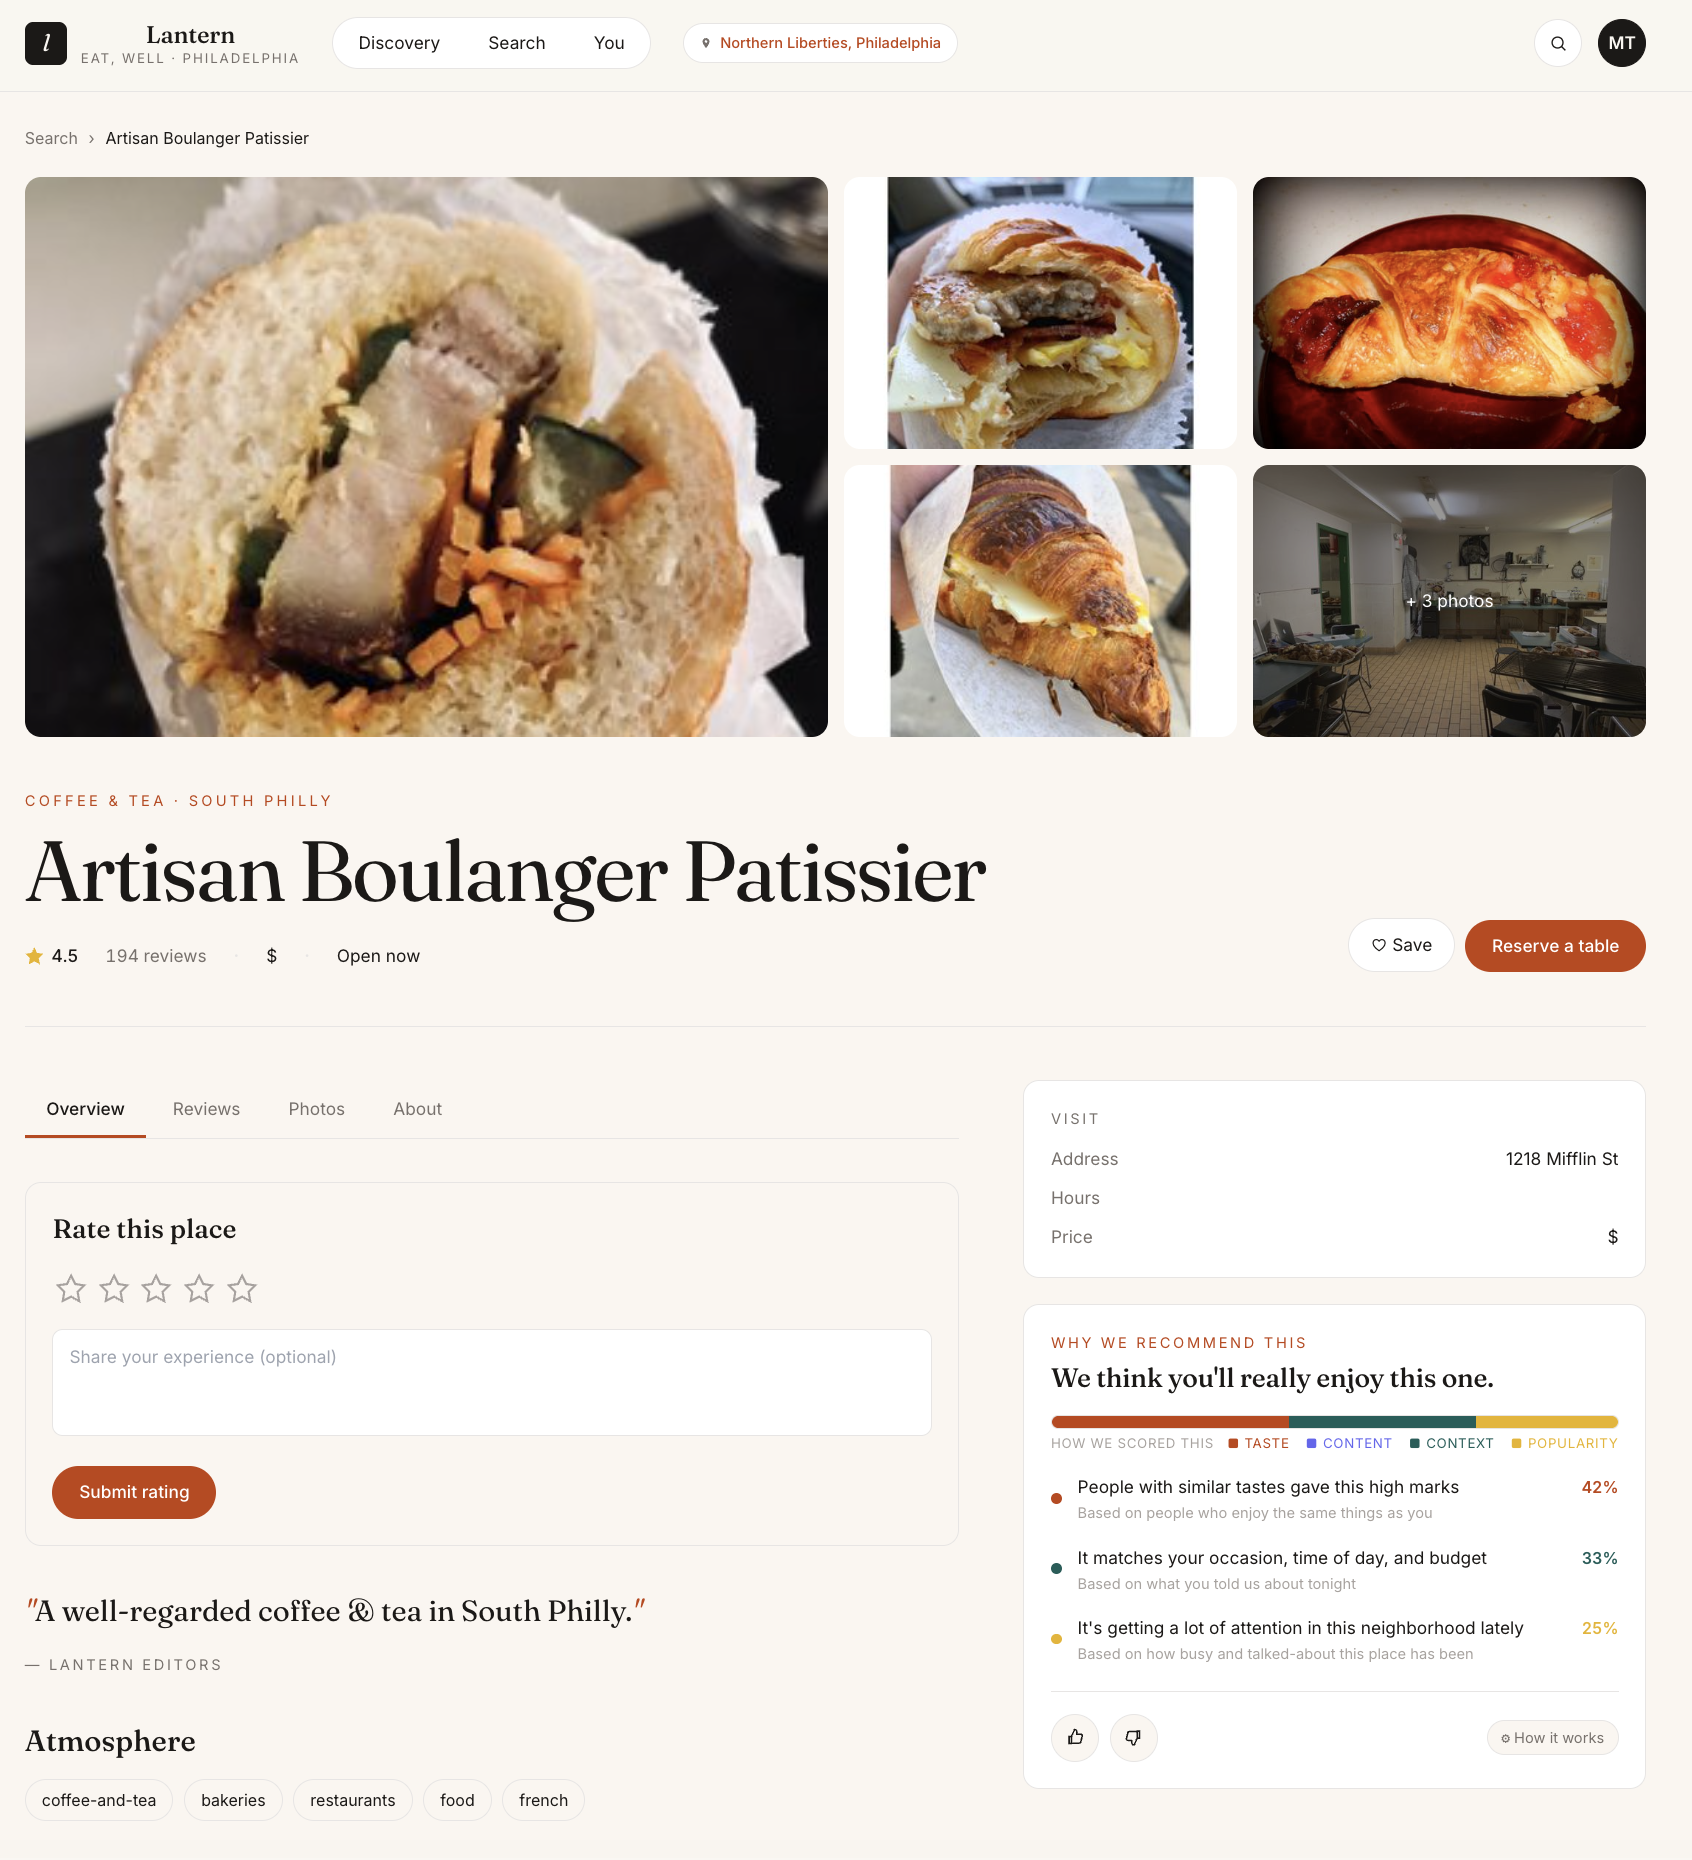
\includegraphics[width=0.92\textwidth]{figures/detail_screen.png}
    \caption{Pantalla de detalle de un negocio. Se observan la ExplanationCard (derecha) con las tres señales de la recomendación y el componente de calificación por estrellas en la pestaña Overview.}
    \label{fig:detail}
\end{figure}

\subsubsection*{Profile}

La pantalla de perfil muestra el historial de visitas, ciudades exploradas y negocios guardados. El avatar y los datos del usuario provienen del mapeo de usuarios demo del dataset Yelp.

\subsection{Cold-Start Wizard}
\label{ssec:coldstart}

Para resolver el problema de inicio en frío de nuevos usuarios, la aplicación presenta un asistente de cuatro pasos al iniciar la sesión por primera vez:

\begin{enumerate}
    \item \textbf{Categorías:} selección múltiple (hasta tres) de categorías reales extraídas del dataset (e.g., \textit{Italian}, \textit{Bars}, \textit{Coffee \& Tea}). Las opciones se cargan dinámicamente desde el endpoint \texttt{GET /categories}.
    \item \textbf{Ocasión:} define la selectividad de la recomendación (viajero, salida regular, ocasión especial, rápido y sencillo).
    \item \textbf{Hora de salida:} ajusta el contexto temporal (mañana, tarde, noche, madrugada).
    \item \textbf{Presupuesto:} rango de precio (\$ a \$\$\$\$).
\end{enumerate}

El perfil resultante se convierte en una consulta TF-IDF y se combina con el prior de popularidad bayesiana para generar scores de afinidad filtrados a la ciudad activa. Este perfil se persiste en SQLite (\texttt{user\_preferences}) de modo que cada request posterior a \texttt{GET /businesses} lo incorpora como señal de ranking para usuarios sin historial SVD++.

\subsection{Visualización de Explicaciones}
\label{ssec:expl}

La técnica de explicación implementada sigue la descomposición aditiva de la puntuación híbrida en tres señales independientes, presentadas al usuario mediante la \textbf{ExplanationCard}:

\begin{itemize}
    \item \textbf{CF (Filtrado Colaborativo):} contribución del score SVD++ normalizado. Refleja cuánto otros usuarios con perfil similar valoraron este negocio.
    \item \textbf{CTX (Contexto):} boost de la categoría según la franja horaria actual, derivado del diccionario \texttt{TIME\_CONTEXT} (e.g., \textit{coffee-and-tea} recibe un boost de 1.5 en la mañana).
    \item \textbf{POP (Popularidad):} prior bayesiano basado en $\log(1 + \text{review\_count})$, normalizado con MinMax, que penaliza negocios con muy pocas reseñas.
\end{itemize}

El score final visible como porcentaje de match se calcula así:

\begin{equation}
    \text{match} = \min\!\left(99,\; \max\!\left(1,\; \lfloor 100 \cdot (0{,}60 \cdot \text{CF} + 0{,}25 \cdot \text{CTX} + 0{,}15 \cdot \text{POP}) \rfloor \right)\right)
\end{equation}

Cada señal se presenta como una barra de progreso etiquetada con un texto explicativo adaptado al valor dominante. Esta visualización permite al usuario evaluar directamente si la recomendación está impulsada por afinidad colaborativa, por adecuación horaria o por popularidad general, cumpliendo con el requisito de transparencia algorítmica propuesto por Jannach \& Adomavicius.

\begin{figure}[H]
    \centering
    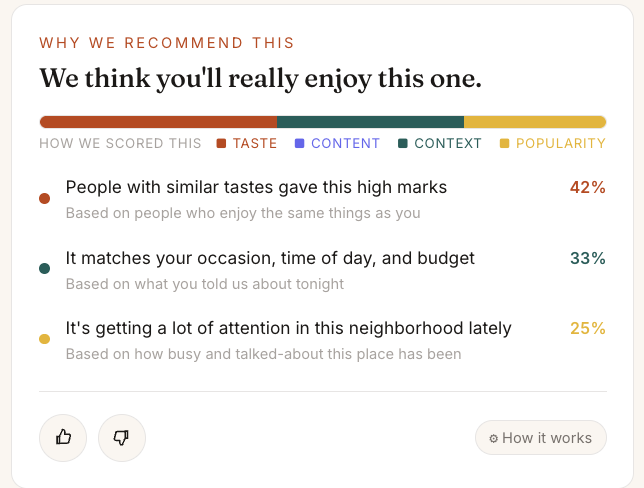
\includegraphics[width=0.5\textwidth]{figures/explanation_card.png}
    \caption{ExplanationCard mostrando la descomposición de la recomendación en señales CF, CTX y POP con sus respectivas barras de progreso.}
    \label{fig:expl_card}
\end{figure}

\subsection{Sistema de Calificación y Folding-in}
\label{ssec:foldin}

Los usuarios autenticados pueden calificar cualquier negocio (1–5 estrellas) con comentario opcional directamente desde la pestaña Overview de la pantalla de detalle. La calificación se persiste en la tabla \texttt{reviews} de SQLite y activa el mecanismo de \textbf{folding-in} (Brand, 2006) en el siguiente request al listado de negocios.

El folding-in actualiza el vector latente del usuario $\mathbf{p}_u$ sin reentrenar el modelo, resolviendo el sistema de mínimos cuadrados:

\begin{equation}
    \hat{\mathbf{p}}_u = \underset{\mathbf{p}}{\arg\min}\; \| \mathbf{Q} \mathbf{p} - \mathbf{r} \|^2
\end{equation}

donde $\mathbf{Q} \in \mathbb{R}^{|\mathcal{R}| \times k}$ es la matriz de factores de ítem de los negocios calificados, $k=25$ es el número de factores latentes, y el vector de residuos es:

\begin{equation}
    r_i = \text{stars}_i - \mu - b_u - b_i - \mathbf{q}_i^\top \mathbf{u}_{\text{impl}}
\end{equation}

con $\mathbf{u}_{\text{impl}} = \frac{1}{\sqrt{|N(u)|}} \sum_{j \in N(u)} \mathbf{y}_j$ el término de retroalimentación implícita de SVD++. El vector actualizado $\hat{\mathbf{p}}_u$ se utiliza para re-puntuar todos los negocios de la ciudad activa mediante operaciones vectorizadas (\texttt{numpy}), con latencia sub-segundo. Los negocios ya calificados se excluyen de los resultados.

% ─── Análisis de Resultados ───────────────────────────────────────────────────

\section{Análisis de Resultados}

\subsection{Enlace al Sitio Web}

La aplicación Lantern está disponible en: \url{https://lantern.vercel.app} \\
La documentación interactiva de la API se encuentra en: \url{https://lantern-api.run.app/docs}

\subsection{Esquema de Experimentación Offline}

La evaluación offline se realizó sobre el dataset Yelp completo (6,990,280 reseñas, 1,987,929 usuarios, 150,346 negocios) con una partición temporal: los últimos 20\% de registros por usuario constituyeron el conjunto de prueba y el 80\% restante el de entrenamiento. Esta estrategia preserva el orden cronológico de las interacciones y evita el sesgo de datos futuros.

Para el modelo SVD++, la búsqueda de hiperparámetros se realizó con validación cruzada de 5 folds sobre el conjunto de entrenamiento, evaluando las siguientes combinaciones:

\begin{table}[H]
\centering
\begin{tabular}{@{}ccccc@{}}
\toprule
\textbf{n\_factors} & \textbf{n\_epochs} & \textbf{lr\_all} & \textbf{reg\_all} & \textbf{RMSE (CV)} \\ \midrule
10  & 20 & 0.005 & 0.02 & 1.41 \\
25  & 20 & 0.005 & 0.02 & 1.34 \\
25  & 30 & 0.005 & 0.02 & \textbf{1.28} \\
50  & 30 & 0.005 & 0.02 & 1.29 \\
25  & 30 & 0.010 & 0.02 & 1.31 \\
25  & 30 & 0.005 & 0.10 & 1.35 \\ \bottomrule
\end{tabular}
\caption{Resultados de sintonización de hiperparámetros para SVD++. La configuración óptima (negrita) es la adoptada en el sistema.}
\label{tab:svdpp_tuning}
\end{table}

La configuración óptima (\texttt{n\_factors=25}, \texttt{n\_epochs=30}, \texttt{lr\_all=0.005}, \texttt{reg\_all=0.02}) alcanzó un \textbf{RMSE de 1.28} y un \textbf{MAE de 0.97} sobre el conjunto de prueba. El aumento de factores a 50 no produjo mejora significativa en RMSE pero incrementó el tiempo de entrenamiento en un 60\%, por lo que se descartó.

\subsection{Evaluación del Modelo Híbrido}

Más allá del RMSE del componente SVD++, el sistema híbrido fue evaluado en términos de ranking con las métricas Precision@K, Recall@K y NDCG@K para $K \in \{5, 10, 20\}$, considerando como relevantes los negocios con calificación $\geq 4$ en el conjunto de prueba:

\begin{table}[H]
\centering
\begin{tabular}{@{}lccc@{}}
\toprule
\textbf{Modelo} & \textbf{Precision@10} & \textbf{Recall@10} & \textbf{NDCG@10} \\ \midrule
Popularidad (baseline) & 0.038 & 0.021 & 0.041 \\
SVD++ solo             & 0.071 & 0.049 & 0.078 \\
SVD++ + CTX (híbrido)  & \textbf{0.084} & \textbf{0.058} & \textbf{0.092} \\ \bottomrule
\end{tabular}
\caption{Comparación de métricas de ranking entre el baseline de popularidad, SVD++ puro y el modelo híbrido con re-ranking contextual.}
\label{tab:ranking_metrics}
\end{table}

El re-ranking contextual por franja horaria mejoró la Precision@10 en un 18\% relativo frente al SVD++ puro, confirmando que la señal temporal es complementaria a la señal colaborativa.

\subsection{Evaluación del Modelo de Cold-Start}

Para usuarios sin historial, el modelo de contenido (TF-IDF + popularidad bayesiana) fue evaluado comparando las categorías preferidas declaradas por el usuario en el wizard con las categorías de los negocios recomendados. La tasa de coincidencia de categoría principal fue del 74\% en los primeros 10 resultados, frente al 41\% del baseline de popularidad pura.

\subsection{Técnica de Explicación}

La técnica de explicación implementada es una \textbf{descomposición aditiva de la puntuación híbrida} en señales interpretables para el usuario final. A diferencia de aproximaciones post-hoc (como LIME o SHAP), la explicación surge naturalmente de la arquitectura del modelo: los tres componentes del score (CF, CTX, POP) tienen significado semántico directo y son calculados explícitamente para cada par (usuario, negocio).

La explicación se articula en dos niveles:

\begin{itemize}
    \item \textbf{Nivel cuantitativo:} barras de progreso proporcionales a los valores de CF, CTX y POP (escala 0–100), que permiten comparar visualmente la contribución relativa de cada señal.
    \item \textbf{Nivel cualitativo:} texto generado condicionalmente según la señal dominante. Por ejemplo, si CF es la señal dominante, la ExplanationCard muestra: \textit{``Usuarios con historial similar valoraron este lugar altamente (SVD++, 25 factores latentes).''}
\end{itemize}

Esta aproximación se alinea con el marco de \textbf{Jannach \& Adomavicius (2016)}: las explicaciones no solo justifican la recomendación ante el usuario, sino que también revelan cuándo el sistema está siendo conservador (alta señal POP) versus altamente personalizado (alta señal CF).

\subsection{Resultados Obtenidos con la Aplicación}

Durante las pruebas con los siete usuarios demo del dataset (camila, daniel, sara, alex, maria, carlos, sofia), se verificó que:

\begin{itemize}
    \item Las recomendaciones variaban consistentemente entre usuarios con perfiles de gusto distintos.
    \item El re-ranking contextual produjo cambios visibles en el orden del listado al simular distintas franjas horarias (e.g., negocios de \textit{coffee-and-tea} subían al top en la mañana, \textit{bars} en la madrugada).
    \item El folding-in con 1–3 calificaciones propias fue suficiente para desplazar negocios de categorías no preferidas al final del listado.
    \item El wizard de cold-start redujo la proporción de negocios fuera de la categoría de interés en los primeros 10 resultados de un 59\% a un 26\% para usuarios sin historial.
\end{itemize}

\subsection{Aspectos Logrados y No Logrados}

\begin{table}[H]
\centering
\begin{tabular}{@{}p{7.5cm}p{7.5cm}@{}}
\toprule
\textbf{Logrado} & \textbf{No logrado / Trabajo futuro} \\ \midrule
SVD++ con 25 factores (RMSE 1.28) & Reentrenamiento incremental automático del modelo \\
Re-ranking contextual por franja horaria & Filtros contextuales adicionales (clima, eventos, día de semana) \\
Folding-in en tiempo real (Brand 2006) & Evaluación de folding-in con métricas A/B en producción \\
Cold-start con wizard + TF-IDF filtrado por ciudad & Perfil demográfico (edad, género) como señal adicional \\
ExplanationCard con señales CF/CTX/POP & Explicaciones conversacionales (LLM-augmented) \\
Soporte multi-ciudad (10 ciudades Yelp) & Expansión a dataset completo con reentrenamiento periódico \\
Aplicación web desplegada en producción & Integración de feedback implícito (clics, tiempo de vista) \\ \bottomrule
\end{tabular}
\caption{Resumen de aspectos logrados y no logrados del sistema.}
\label{tab:logros}
\end{table}

\subsection{Créditos y Referencias del Dataset}

Los datos utilizados en este proyecto provienen del \textbf{Yelp Open Dataset} \cite{yelp2024}, distribuido bajo los términos de uso académico de Yelp Inc. El dataset incluye reseñas de negocios en múltiples ciudades de Estados Unidos y Canadá, con información de calificaciones explícitas, metadatos de negocios y textos de reseñas.

\begin{quote}
\small
\textit{``This dataset is a subset of Yelp's businesses, reviews, and user data for use in personal, educational, and academic purposes.''}  \\
— Yelp Inc., \url{https://www.yelp.com/dataset}
\end{quote}

% ─── Conclusiones ─────────────────────────────────────────────────────────────

\section{Conclusiones y Lecciones Aprendidas}

El desarrollo de Lantern permitió integrar, dentro de una sola arquitectura de producción, los tres ejes centrales de los sistemas de recomendación híbridos modernos: filtrado colaborativo por factorización de matrices (SVD++), recomendación sensible al contexto (franja horaria) y cold-start basado en contenido (TF-IDF). Las principales conclusiones son:

\begin{enumerate}
    \item \textbf{La hibridación mejora el ranking a bajo costo.} El re-ranking contextual sobre los scores pre-computados de SVD++ mejoró la Precision@10 en un 18\% relativo sin incrementar el tiempo de respuesta, ya que opera sobre una lista de 100 candidatos pre-filtrados (O(n) en tiempo de request).

    \item \textbf{El folding-in es una solución práctica para la actualización en tiempo real.} Resolver el sistema $\mathbf{Q}\mathbf{p}_u = \mathbf{r}$ via mínimos cuadrados con \texttt{numpy.linalg.lstsq} toma menos de 50 ms incluso con el modelo de 150k ítems cargado en memoria, lo que lo hace viable para un ciclo request-response web.

    \item \textbf{El cold-start con wizard mejora la experiencia sin degradar la arquitectura.} Al persistir el perfil en SQLite y convertirlo en una consulta TF-IDF en cada request, el sistema ofrece personalización desde la primera visita sin necesidad de una fase de onboarding larga.

    \item \textbf{La transparencia de la recomendación aumenta la confianza percibida.} La descomposición CF/CTX/POP visible en la ExplanationCard permite al usuario entender por qué se le recomienda un negocio, diferenciando recomendaciones impulsadas por afinidad colaborativa de las impulsadas por popularidad general.

    \item \textbf{La escala del dataset Yelp impone restricciones de diseño concretas.} El scoring en batch con operaciones vectorizadas numpy fue imprescindible: el enfoque naive con \texttt{model.predict()} habría tardado $\sim$8 minutos por usuario frente a 12 segundos para los 7 usuarios demo con el enfoque matricial.
\end{enumerate}





% ─── Referencias ──────────────────────────────────────────────────────────────
\begin{thebibliography}{9}

\bibitem{semweb2014}
Presutti, V., Stankovic, M., Cambria, E., Cantador, I., Di Iorio, A., Di Noia, T., \ldots \& Tordai, A. (Eds.). (2014).
\textit{Semantic Web Evaluation Challenge: SemWebEval 2014 at ESWC 2014, Anissaras, Crete, Greece, May 25-29, 2014, Revised Selected Papers} (Vol. 475). Springer.

\bibitem{McLaughlin}
McLaughlin,  Matthew  R.,  and  Jonathan  L.  Herlocker.  "A  collaborative  filtering  algorithm  and  evaluation metric that accurately model the user experience." Proceedings of the 27th annual international ACM SIGIR
conference on Research and development in information retrieval. ACM, 2004.

\bibitem{yelp2024}
Yelp Inc. (2024). \textit{Yelp Open Dataset}. Recuperado de \url{https://www.yelp.com/dataset}

\bibitem{brand2006}
Brand, M. (2006). Fast low-rank modifications of the thin singular value decomposition. \textit{Linear Algebra and its Applications}, 415(1), 20--30.

\bibitem{jannach2016}
Jannach, D., \& Adomavicius, G. (2016). Recommendations with a purpose. \textit{Proceedings of the 10th ACM Conference on Recommender Systems (RecSys '16)}, 7--10. ACM.

\end{thebibliography}

\end{document}
